\section{Supervised Learning and Generalisation}

\subsection{The Perceptron}

\subsubsection{Linear Regression with a Perceptron}

A perceptron with linear activation \eqref{eq:perceptron}
and MSE
is equivalent to linear regression \eqref{eq:linear-regression}:

\begin{equation}
    y \approx f(x; w_1, \dots, w_N, b) =  \sigma \big( \sum_{i=1}^N{w_i x_i} + b \big), \,
    \sigma \in \{ \textit{linear} \} \notin \{ \tanh, \textit{sigmoid}, \textit{sign}, \dots \}
    \label{eq:perceptron}
\end{equation}

\begin{equation}
    y \approx f(x; w_1, \dots, w_N, b) = \sum_{i=1}^N{w_i x_i} + b, \quad
    {\arg \min}_{w_1, \dots, w_N, b}{ \big( y - f(x; w_1, \dots, w_N, b) \big)^2 }
\label{eq:linear-regression}
\end{equation}

\subsubsection{Linear Models}

A linear model $\sum_{i=1}^N{w_i x_i} + b$ is \textit{linear} in the parameters \citep{deisenroth2020mathematicsforml}
(and bias) $w_1, \dots, w_N, b$, but may be nonlinear in the features,
e.g. polynomial regression with features $x, x^2, \dots$, or some basis functions -
which would be able to capture sinusoidal data (perfectly).

A perceptron only captures linear relationships; and underfits sinusoidal data.
A MLP
with nonlinear activations and
multiple layers of (a sufficient number of) hidden neurons, however,
e.g. $f = W \sigma\big(H_2 \sigma(H_1 x + b_1) + b_2\big)$,
is a universal function approximator. \citep{HORNIK1989359}

Moreover, the approximation error for an MLP, $\mathcal{O}(\frac{1}{n_h})$,
depends on the no. of hidden units but \textit{not} on the input space dimension $n$ -
unlike for polynomial expansions, $\mathcal{O}(\frac{1}{n_p^{\frac{2}{n}}})$.

\subsubsection{The Effect of the Learning Rate}
\label{subsubsection:learning-rate}

A small learning rate $\eta$ causes gradient descent to take smaller steps, while a large $\eta$ causes it to take bigger steps.
Consequently, with a smaller learning rate, training loss decreases more slowly and gradient descent converges more slowly;
if $\eta$ is too large it may not converge.
The experiments validate this empirically, e.g. with $\eta = 0.002, 0.2, 2.0$.

Learning rate decay\footnote{
    An alternative to learning rate decay / scheduling is to gradually increase the batch size. \citep{smith2017dontdecaythelearningrate}
    Increasing the batch size reduces gradient noise, which similarly facilitates optimisation.
    Although in general, the batch size cannot be changed blindly as it alters the training dynamics, and
    requires tuning hyperparameters like effective learning rate and regularisation accordingly.
    \citep{tuningplaybookgithub}
} \citep{you2019doeslearningratedecay} and
adaptive optimisers like Adam \citep{kingma2017adammethodstochasticoptimization}
(larger updates for parameters with smaller gradients, smaller updates for parameters with larger gradients)
adapt the learning rate during training - with the aim of speeding up convergence.

\subsubsection{The Loss Curve}

With a larger learning rate, mini-batches give a noisy estimate\footnote{
    SGD updates are noisy but unbiased; i.e. convergence in expectation - with a suitable learning rate.
} of the gradient for SGD.
Adam's adaptive learning rates result in some larger or smaller steps.

\subsection{Backprop}

Backpropagation recursively propagates the error from the output back to the input.


\subsection{Training Algorithms}
\label{subsection:training-algorithms}

\subsubsection{The Effect of Noise on the Optimisation Process}

"Injecting noise \dots [is] a form of data augmentation" \citep{SIETSMA199167,Goodfellowetal2016}
although "neural networks prove not to be very robust to noise". \citep{TangE10,Goodfellowetal2016}
The model still achieves good training and validation loss values after 15 to 25 epochs.
When trained on pure noise, loss remains high (i.e. not learning much signal); from 20 epochs it starts overfitting the noise somewhat.

\begin{figure}[h!]
    \begin{minipage}[t]{0.32\textwidth}
        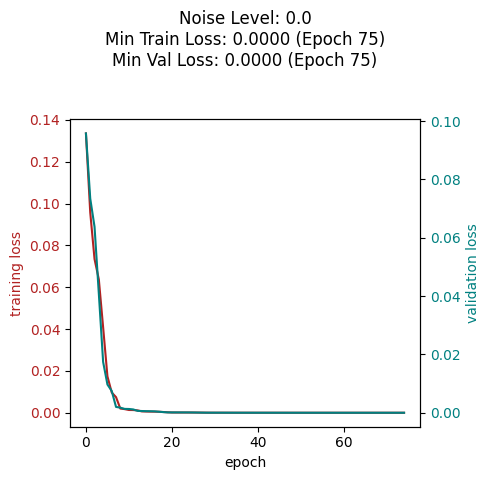
\includegraphics[width=\textwidth]{figures/noise-level-0-0.png}
        \label{fig:noise-level-0-0}
    \end{minipage}
    \begin{minipage}[t]{0.32\textwidth}
        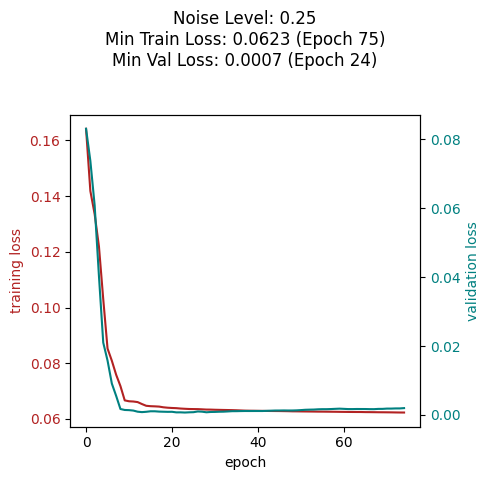
\includegraphics[width=\textwidth]{figures/noise-level-0-25.png}
        \label{fig:noise-level-0-25}
    \end{minipage}
    \begin{minipage}[t]{0.32\textwidth}
        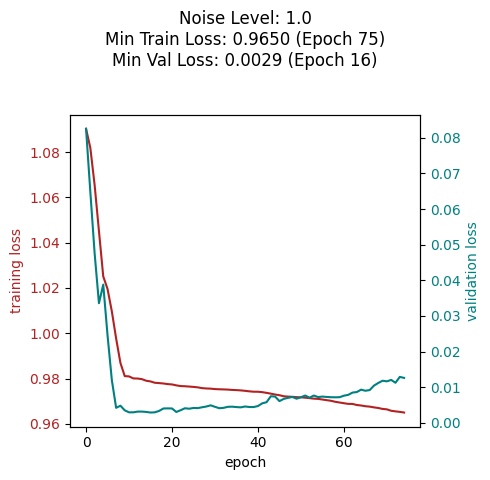
\includegraphics[width=\textwidth]{figures/noise-level-1-0.png}
        \label{fig:noise-level-1-0}
    \end{minipage}
    \vspace{-20pt}
    \caption{L-BFGS training and validation loss curves with 0 vs. 25 vs. 100\% noise}
\end{figure}

Noise, e.g. $\epsilon \sim \mathcal{N}(0, \sigma^2), \epsilon \perp g$,
affects the gradients, $\tilde{g} = g + \epsilon$:
unbiased, $\mathbb{E}[\tilde{g}] = g$,
but higher \textit{gradient} variance, $Var(\tilde{g}) = Var(g) + Var(\epsilon)$.
Some noise may act as regularisation \textit{and} improve optimisation \citep{neelakantan2015addinggradientnoiseimproves}
with gradient variance often yielding better generalisation, avoiding local minima;
too much noise makes training unstable (Figure \ref{fig:noise-level-1-0-num-layers-3-num-units-50}, cf. SGD\footnote{
    Small batches, esp. SGD, often act as regularisation at the cost of stability, runtime (smaller $\eta$). \citep{Goodfellowetal2016}
}).

\subsubsection{GD vs. SGD vs. AGD vs. Adam vs. L-BFGS}
\label{subsubsection:gd-vs-sgd-vs-agd-vs-adam-vs-lbfgs}

Full-batch gradient descent is guaranteed to decrease the loss on every iteration
with a sufficiently small learning rate, i.e. $\eta < 2 / L$,
for a Lipschitz-smooth convex function.
Stochastic mini-batch gradient descent exhibits stochastic gradient updates
based on a mini-batch of the full data and oscillates (more, depending on the batch size).
Adaptive methods and second-order approximations are designed to accelerate convergence:
Adam \citep{kingma2017adammethodstochasticoptimization}, RMSProp \citep{hinton2012rmsprop} and Adadelta \citep{zeiler2012adadeltaadaptivelearningrate}
do so by adapting the learning rate using gradient moments,
or running averages of past gradients, respectively.
NAG \citep{nesterov1983method} is momentum-based with a look-ahead strategy.\footnote{
    Loss spikes in the first epochs may require learning rate warm-up, or reducing batch size.
}
Limited-memory BFGS \citep{byrd1995limited} is quasi-Newton: it approximates the Hessian
\& uses line search to determine optimal step size.

\begin{figure}[h!]
    \begin{minipage}[t]{0.32\textwidth}
        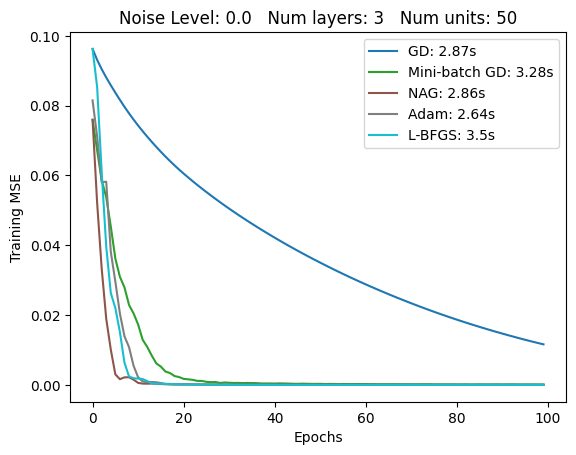
\includegraphics[width=\textwidth]{figures/noise-level-0-0-num-layers-3-num-units-50.png}
        \label{fig:noise-level-0-0-num-layers-3-num-units-50}
    \end{minipage}
    \begin{minipage}[t]{0.32\textwidth}
        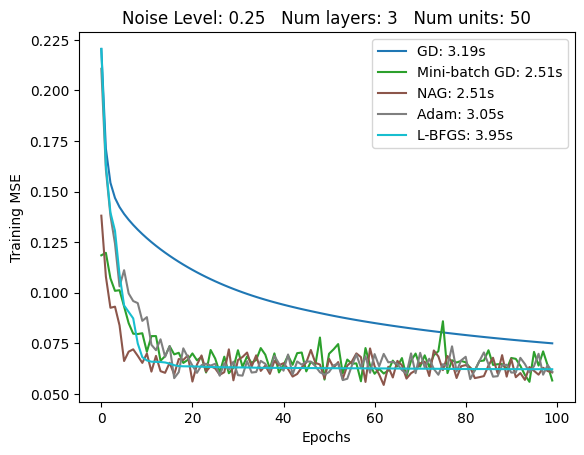
\includegraphics[width=\textwidth]{figures/noise-level-0-25-num-layers-3-num-units-50.png}
        \label{fig:noise-level-0-25-num-layers-3-num-units-50}
    \end{minipage}
    \begin{minipage}[t]{0.32\textwidth}
        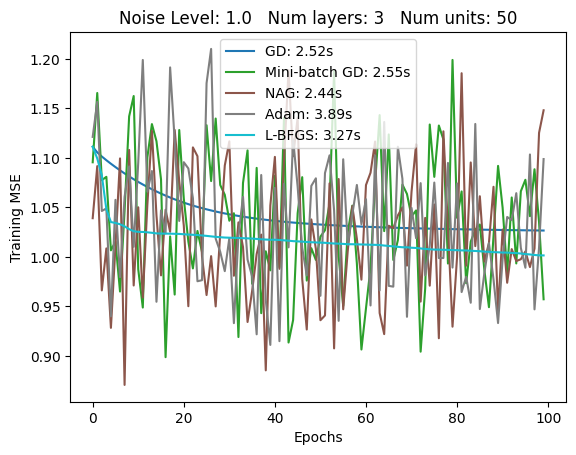
\includegraphics[width=\textwidth]{figures/noise-level-1-0-num-layers-3-num-units-50.png}
        \label{fig:noise-level-1-0-num-layers-3-num-units-50}
    \end{minipage}
    \vspace{-20pt}
    \caption{GD, mini-batch GD, NAG, Adam, L-BFGS loss with 0 vs. 25 vs. 100\% noise}
\end{figure}

\subsubsection{Impact of Network Size on the Choice of Optimizer}

\vspace{-2.5pt}
The larger the size of the network, the better Adam and mini-batch GD perform
compared with NAG and L-BFGS. Also full-batch GD performs better for larger networks.
\vspace{-2.5pt}

\begin{figure}[h!]
    \begin{minipage}[t]{0.32\textwidth}
        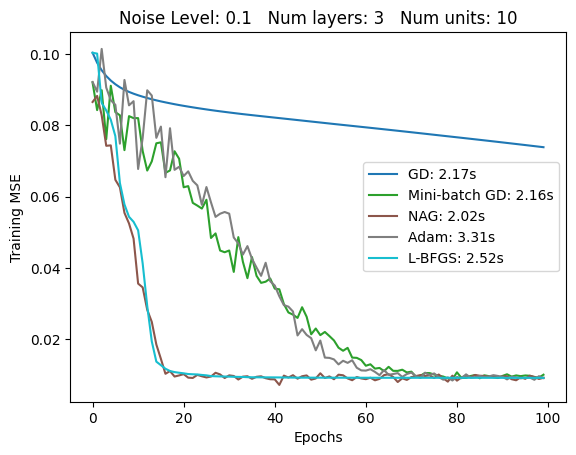
\includegraphics[width=\textwidth]{figures/noise-level-0-1-num-layers-3-num-units-10.png}
        \label{fig:noise-level-0-1-num-layers-3-num-units-10}
    \end{minipage}
    \begin{minipage}[t]{0.32\textwidth}
        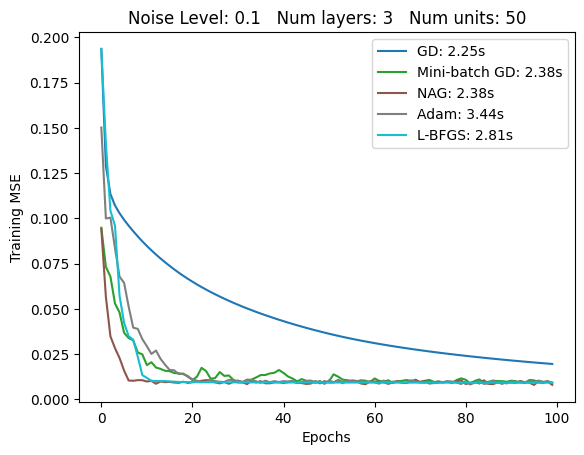
\includegraphics[width=\textwidth]{figures/noise-level-0-1-num-layers-3-num-units-50.png}
        \label{fig:noise-level-0-1-num-layers-3-num-units-50}
    \end{minipage}
    \begin{minipage}[t]{0.32\textwidth}
        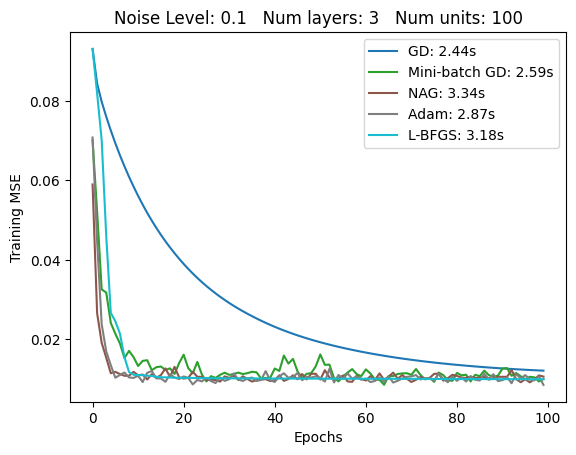
\includegraphics[width=\textwidth]{figures/noise-level-0-1-num-layers-3-num-units-100.png}
        \label{fig:noise-level-0-1-num-layers-3-num-units-100}
    \end{minipage}
    \vspace{-15pt}
    \caption{GD, mini-batch GD, NAG, Adam, L-BFGS loss with 10 vs. 50 vs. 100 neurons}
    \vspace{-2.5pt}
\end{figure}

\vspace{-15pt}

\subsubsection{Epochs, Time and Convergence}

An epoch is one pass through the training data, with $1 \leq \lvert \text{batch} \rvert \leq \, \lvert \text{training data} \rvert$.
Time is the actual time taken, depending on the optimiser, hardware, etc., and on the batch size.
Convergence occurs at the point where the objective stabilises and/or does not improve further.
Speed of convergence may thus be in terms of no. of epochs or time.
In practice it is training \textit{time} that matters (and computation, cf. e.g. Newton's method).

GD shows poor convergence speed in time and no. of epochs.
The other algorithms converge well in time, no. of epochs, although mini-batch GD may require more epochs.


\subsubsection{Parametrisation of a Convolutional Neural Network (CNN)}

The CNN comprises two convolutional blocks (each with a conv and max pooling layer),
followed by a flattening, dropout, and dense output layer.
Each conv layer uses a kernel with specified height, width, input channels, and output filters, plus one bias per filter.
Pooling layers downsample the feature maps.
The CNN has 34,826 trainable\footnote{
    Non-trainable parameters appear in layers like frozen layers (e.g., when reusing pre-trained embeddings)
    and batch normalisation.
    A batch normalisation layer — insertable between conv and pooling —
    would add trainable scale and shift parameters, and non-trainable running mean and variance.
} parameters.

The first convolution receives input images of shape $28 \times 28 \times 1$, uses a $3 \times 3$ kernel, and outputs $32$ filters: $(3 \times 3 \times 1 \times 32) + 32 = 320$ parameters ($288$ weights, $32$ biases).
Both pooling layers are $2 \times 2$.
After pooling, the second convolution operates on input of shape $13 \times 13 \times 32$, with the same kernel and $64$ filters: $(3 \times 3 \times 32 \times 64) + 64 = 18,\!496$ parameters.
The output is flattened, a dropout of $0.5$ is applied, and a final dense softmax layer maps $1600$ inputs to $10$ outputs, totaling $(1600 \times 10) + 10 = 16,\!010$ params.
\citep{dumoulin2018guideconvolutionarithmeticdeep,zhang2023d2l}

\subsubsection{Training a CNN on MNIST with Adam vs. SGD vs. Adadelta}

With early stopping \footnote{
    Early stopping is performed on validation (categorical cross-entropy) loss, with continuous gradient,
    decreases more smoothly and gives a more stable signal of generalisation than discrete accuracy.
} and restoring best weights,
Adam achieves $\approx 0.9929$ test accuracy (and $\approx 0.0217$ test loss) in 30 epochs,
SGD (with learning rate scheduling) $\approx 0.9909$ (and $\approx 0.0263$) in 43 epochs, and
Adadelta (with tuned learning rate) $\approx 0.9888$ (and $\approx 0.0345$) in 50 epochs.
Further hyperparameter tuning could further improve performance.

Adadelta \citep{zeiler2012adadeltaadaptivelearningrate} (like RMSProp \citep{hinton2012rmsprop}) is a variant of Adagrad \citep{duchi2011adaptive},
computing per-parameter learning rates,
but adapting them less aggressively with "squared \textit{rescaled} gradients". \citep{zhang2023d2l}

\newpage

\subsection{Regression}

\paragraph{Training and Test Split}

The dataset is shown in Figure \ref{fig:regression-splits}.
It is split into a training (second from left) and a test (first from right) set
by randomly sampling without replacement s.t. no point is in both.
Such an independent, identically distributed test set
(i.i.d., i.e. sampled from the same distribution but may not overlap with the training data)
is needed to evaluate a model's capabilities of generalisation to unseen, out-of-sample data.

\begin{figure}[h!]
    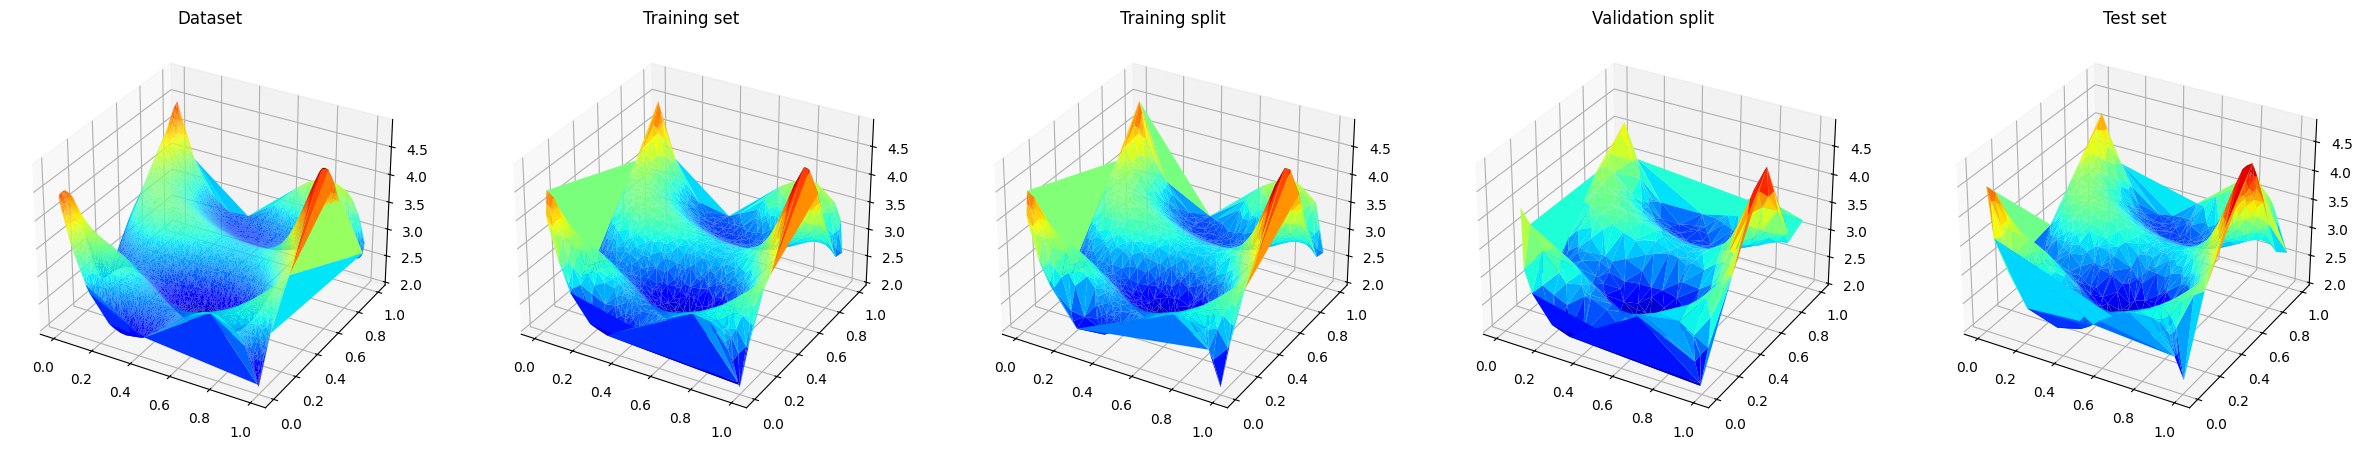
\includegraphics[width=\textwidth]{figures/regression-splits.png}
    \caption{Dataset, training set (with training and validation splits), test set}
    \label{fig:regression-splits}
\end{figure}
\vspace{-10pt}

\paragraph{Model Selection}

For model selection, a grid search is used, as the space is not too large:
Adam with a fixed learning rate is used as a default to run a grid search on the number of layers and neurons and activation function; finally learning rate, optimiser, etc. are tuned.
To validate the model, the training set from the initial split (second from left, in Figure \ref{fig:regression-splits}) is split further, into a training set (third) and a validation set (fourth).

A shallow network (i.e. with one single hidden layer) and unbounded activations in theory is sufficient as a universal approximator for a continuous nonlinear function \citep{prince2023understanding}.
However, a deep network is more efficient (i.e. less complexity) at representing a function, e.g. by utilising hierarchical features \citep{telgarsky2016benefitsdepthneuralnetworks}
at the expense of potentially more time and difficulties (e.g. vanishing gradients) to train.
Two layers with 20 neurons work well here.

\paragraph{Model Evaluation}

No further training is possible in validation-based model selection because, by definition, the model is selected based on the validation set and only evaluated on the test set.
This prevents data leakage and enables evaluation on unseen data.

\begin{figure}[h!]
    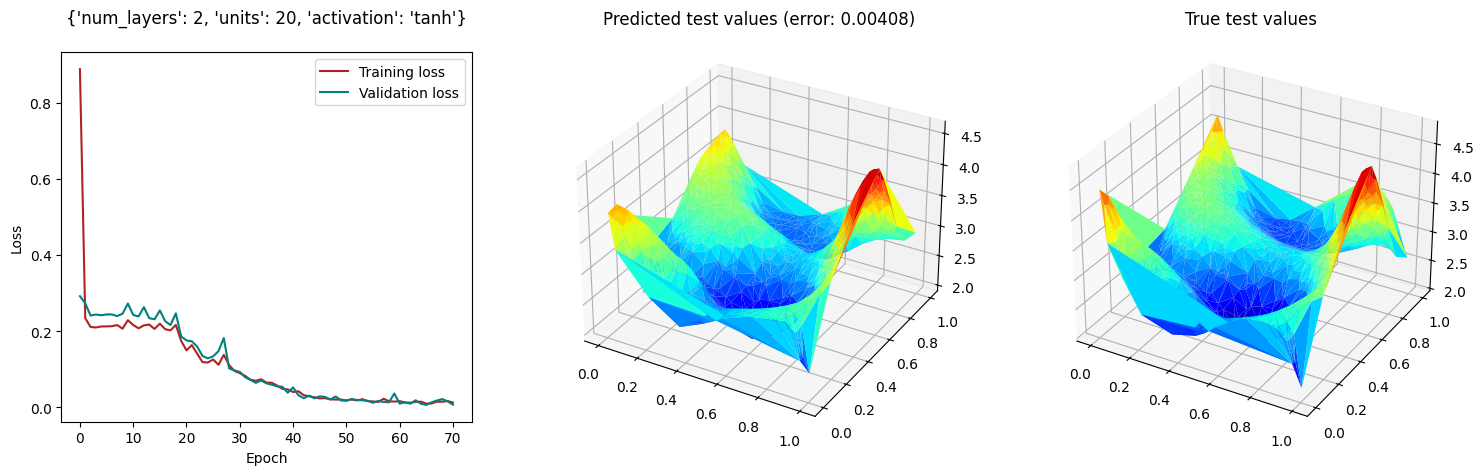
\includegraphics[width=\textwidth]{figures/regression-results.png}
    \caption{Training and validation loss curves, and prediction on test set (MSE: $0.004$)}
    \label{fig:regression-results}
\end{figure}
\vspace{-10pt}

\paragraph{Overfitting and Regularisation}

Regularisation reduces a model's flexibility by penalising large or complex parameters, and
thereby lowering its effective number of parameters or degrees of freedom.
Here, early stopping is used to prevent overfitting - as evidenced on the test set (Figure \ref{fig:regression-results}).
L1 / L2 and dropout are other common methods.
